\chapter{Arhitektura i dizajn sustava}
		\begin{comment}
		\textbf{\textit{dio 1. revizije}}\\

		\textit{ Potrebno je opisati stil arhitekture te identificirati: podsustave, preslikavanje na radnu platformu, spremišta podataka, mrežne protokole, globalni upravljački tok i sklopovsko-programske zahtjeve. Po točkama razraditi i popratiti odgovarajućim skicama:}
	\begin{itemize}
		\item 	\textit{izbor arhitekture temeljem principa oblikovanja pokazanih na predavanjima (objasniti zašto ste baš odabrali takvu arhitekturu)}
		\item 	\textit{organizaciju sustava s najviše razine apstrakcije (npr. klijent-poslužitelj, baza podataka, datotečni sustav, grafičko sučelje)}
		\item 	\textit{organizaciju aplikacije (npr. slojevi frontend i backend, MVC arhitektura) }		
	\end{itemize}
	\end{comment}
	
		
	Aplikacija je napravljena u Flutteru koji je Googleov open-source framework za izradu aplikacija za više platformi iz jednog programskog koda. 
	Programski jezik koji se koristi u Flutteru je Dart koji ima objektno orijentiranu prirodu, ali je uz to prilagođen za izradu UI-a. 
	Sama arhitektura sustava slična je MVC modelu. \\ 
	Postoji Model napravljen na temelju objektno orijentiranog programiranja, a poistovjećen je s dokumentima u odgovarajućim kolekcijama u bazi podataka. \\
	Uz Model postoji i View čija je svrha prikazati svaki ekran koristeći podatke dobivene iz Modela.
	Ta dva dijela povezana su funkcijama tamo gdje su podatci statički, odnosno Streamovima gdje se podatci mijenjaju, bilo akcijom trenutnog korisnika ili nekog drugog korisnika čija akcija utječe na trenutno izvođenje aplikacije. 
	Stream je također vrsta arhitekture koja se koristi u Flutteru, a povezuje View i Model na način da kad god dođe do promjene u Modelu, View se automatski ažurira. \\
	Model je tako povezan sa streamom podataka iz baze te se svakom promjenom podataka automatski okine i promjena Modela, što uzrokuje automatsko osvježavanje korisnikovog ekrana s najnovijim podatcima. 
	Arhitekturu čine još i Provideri koji se također često koriste u Flutteru, a njihova je svrha da propagiraju podatke između raznih stranica aplikacije. \\
	Na ovaj načina Controller smo zamijenili Streamovima i Providerima koji nam omogućuju kvalitetan protok informacija kroz čitavu aplikaciju.
		

				
		\section{Baza podataka}

		Baza podataka odabrana za potrebe zadatka je Firebase Firestore. \newline
		Firebase je platforma razvijena od strane Googlea za izradu mobilnih i web aplikacija, a izrazito je dobro podržana za aplikacije pisane u Flutteru. Firestore je \textit{document-oriented} NoSQL baza podataka, zbog čega se ER model prikazan u nastavku u određenoj mjeri razlikuje od realne implementacije u Firebaseu. Onome što bi u bazi podataka modeliranoj prema ER modelu bio jedan redak neke tablice, u Firebaseu je jedan primjerak \textit{document}-a. On je reprezentiran jedinstvenim ključem koji generira sam Firebase, a pripada nekoj sebi nadređenoj kolekciji (eng. \textit{collection}), na neki način istovjetnoj ER entitetu. Svaki \textit{document} može sadržavati proizvoljno mnogo informacija proizvoljnog tipa podataka, povezanih u \textit{collection}, što bi se moglo poistovijetiti s atributima u ER modeliranoj bazi podataka. \newline
		
		Baza podataka ove mobilne aplikacije sastoji se od sljedećih entiteta:
		\begin{itemize}
			\item Korisnik
			\item Skladište
			\item Proizvod
			\item Kategorija
			\item Zapis
			\item Inventura
			\item Provjera
			\item Obavijest
			\item Obavijest o nepodudarnosti
		\end{itemize}
		
			\subsection{Opis tablica}

				 \textit{Napomena: Svi su ID atributi tipa VARCHAR zbog toga što Firebase pri dodavanju novih instanci stvara jedinstveni identifikator - ID, koji je kombinacija slova i znamenki.}
			

				Entitet \textbf{Korisnik} predstavlja svakog registriranog korisnika aplikacije. Sastoji se od atributa: IDKorisnika, ime, prezime, email, lokacija na kojoj je skeniran prvi proizvod pri odabiru proizvoda te uloga koju korisnik ima u skladištu.
				Ovaj entitet povezan je s entitetom Skladište preko atributa IDKorisnika koji je strani ključ u Skladištu kao IDNadležnog odgovarajućeg skladišta. Budući da jedno skladište može imati samo jednog šefa, a svaki šef može biti nadležan za samo jedno skladište, veza je \textit{One-to-One}.
								
				\begin{longtblr}[
					label=none,
					entry=none
					]{
						width = \textwidth,
						colspec={|X[6,l]|X[6, l]|X[20, l]|}, 
						rowhead = 1,
					} %definicija širine tablice, širine stupaca, poravnanje i broja redaka naslova tablice
					\hline \multicolumn{3}{|c|}{\textbf{Korisnik}}	 \\ \hline[3pt]
					\SetCell{LightGreen}IDKorisnika & VARCHAR	&  	jedinstveni identifikator, kombijacija slova i znamenki  	\\ \hline
					ime	& VARCHAR & ime korisnika  	\\ \hline 
					prezime	& VARCHAR & prezime korisnika  	\\ \hline 
					email & VARCHAR & email s kojim se korisnik prijavio u sustav  \\ \hline 
					lokacija & VARCHAR	& ime skladišta u kojem je osoba trenutno, određuje se prema GPS lokaciji koju dohvaća mobitel u trenutku skeniranja prvog artikla (odabira artikla), a za šefove skladište je fiksna prema registraciji 		\\ \hline
					uloga	& VARCHAR & pozicija koju korisnik ima u sustavu, može biti skladištar, šef skladišta ili direktor, odabire se pri registraciji  	\\ \hline  
				\end{longtblr}

				Entitet \textbf{Skladište}, kao što mu ime kaže, reprezentacija je skladišta tvrtke. U njemu su zapisani atributi: IDSkladišta, njegovo u praksi korišteno ime, ID šefa skladišta koji je ondje nadležan, kao i GPS lokacija na kojoj se skladište nalazi.

				\begin{longtblr}[
					label=none,
					entry=none
					]{
						width = \textwidth,
						colspec={|X[6,l]|X[6, l]|X[20, l]|}, 
						rowhead = 1,
					} %definicija širine tablice, širine stupaca, poravnanje i broja redaka naslova tablice
					\hline \multicolumn{3}{|c|}{\textbf{Skladište}}	 \\ \hline[3pt]
					\SetCell{LightGreen}IDSkladišta & VARCHAR & jedinstveni identifikator skladišta \\ \hline
					imeSkladišta & VARCHAR	&  	intuitivni naziv skladišta  	\\ \hline
					\SetCell{LightBlue}IDNadležnog	& VARCHAR & jedinstveni identifikator šefa koji je nadležan za skladište  	\\ \hline 
					GPSLokacija & VARCHAR	& GPS koordinate skladišta, zadaje ih direktor pri kreiranju novog skladišta		\\ \hline
				\end{longtblr}
				
				
				\textbf{Proizvod} je entitet koji sadržava sve važne informacije o proizvodu, kao što su: njegov ID, kratak naziv, malo detaljniji opis te jedinica mjere koja se koristi za proizvod.
				U vezi je s nekoliko entiteta. Jedan od njih je Zapis koji predstavlja "jedno skeniranje" određenog broja istovrsnih proizvoda, a veza je \textit{One-to-Many}. Druga je \textit{Many-to-One} veza s entitetom Provjera, gdje je IDProizvoda ujedno i dio kompozitnog ključa.
				U \textit{Many-to-One} vezi je i s entitetom Obavijest, gdje je IDProizvoda također dio kompozitnog ključa, dok je u \textit{Many-to-One} vezi s entitetom Obavijest o nepodudarnosti samo strani ključ. Strani mu je ključ i IDKategorije iz entiteta Kategorija, povezanog \textit{Many-to-One} vezom, a predstavlja kategoriju u koju se proizvod svrstava.

				\begin{longtblr}[
					label=none,
					entry=none
					]{
						width = \textwidth,
						colspec={|X[6,l]|X[6, l]|X[20, l]|}, 
						rowhead = 1,
					} %definicija širine tablice, širine stupaca, poravnanje i broja redaka naslova tablice
					\hline \multicolumn{3}{|c|}{\textbf{Proizvod}}	 \\ \hline[3pt]
					\SetCell{LightGreen}IDProizvoda & VARCHAR	&  	jedinstveni identifikator proizvoda, čita se iz QR ili bar koda  	\\ \hline
					nazivProizvoda	& VARCHAR & kratak naziv proizvoda, može imati minimalan opis kako bi se razlikovao od drugih (npr. CocaCola Zero 0.5l)  	\\ \hline 
					opisProizvoda & VARCHAR	& malo detaljniji opis proizvoda, u njemu su sadržani prilagođeni podatci (npr. veličina i materijal za odjeću, rok trajanja za hranu i sl.)		\\ \hline
					jedinicaMjere & VARCHAR & jedinica u kojoj se proizvod prodaje, može biti komad, kilogram, metar i sl. \\ \hline
					\SetCell{LightBlue}IDKategorije & VARCHAR & jedinstveni identifikator kategorije kojoj proizvod pripada \\ \hline
				\end{longtblr}

				\textbf{Kategorija} je entitet koji skuži za kategorizaciju proizvoda u određene grupe i podgrupe. Zbog toga ima atribute IDKategorije, nazivKategorije te IDRoditelja, i to na način da je IDRoditelja strani ključ u rekurzivnoj \textit{One-to-many} vezi tako da svako dijete može imati samo jednog roditelja, a roditelj može imati N djece.

				\begin{longtblr}[
					label=none,
					entry=none
					]{
						width = \textwidth,
						colspec={|X[6,l]|X[6, l]|X[20, l]|}, 
						rowhead = 1,
					} %definicija širine tablice, širine stupaca, poravnanje i broja redaka naslova tablice
					\hline \multicolumn{3}{|c|}{\textbf{Kategorija}}	 \\ \hline[3pt]
					\SetCell{LightGreen}IDKategorije & VARCHAR	&  	jedinstveni identifikator kategorije  	\\ \hline
					nazivKategorije	& VARCHAR & kratak naziv kategorije (npr. hrana, mliječni proizvod)  	\\ \hline 
					\SetCell{LightBlue} IDRoditelja & VARCHAR & jedinstveni identifikator kategorije koja joj je nadređena  \\ \hline
				\end{longtblr}

				\textbf{Zapis} predstavlja jedno skeniranje jedne vrste proizvoda (svaki put kada korisnik odabere da želi ažurirati stanje proizvoda, dodaje se novi zapis). Ima atribute IDKorisnika, IDSkladišta, trenutakSkeniranja, ID skeniranog proizvoda, količina koja je skenirana te ID inventure tijekom koje se skeniranje dogodilo.
				Primarni mu je ključ kompozitni, posuđuje IDKorisnika iz Korisnika, IDSkladišta iz Skladišta te IDProizvoda iz Proizvoda. Sadrži i atribut količina te IDInventure koji je posuđen iz entiteta Inventura.
				Veza je \textit{Many-to-One}.

				\begin{longtblr}[
					label=none,
					entry=none
					]{
						width = \textwidth,
						colspec={|X[6,l]|X[6, l]|X[20, l]|}, 
						rowhead = 1,
					} %definicija širine tablice, širine stupaca, poravnanje i broja redaka naslova tablice
					\hline \multicolumn{3}{|c|}{\textbf{Zapis}}	 \\ \hline[3pt]
					\SetCell{LightGreen}IDKorisnika & VARCHAR	&  	jedinstveni identifikator korisnika koji je skenirao proizvod 	\\ \hline
					\SetCell{LightGreen}IDSkladišta & VARCHAR	&  	jedinstveni identifikator skladišta u kojem je proizvod skeniran	\\ \hline
					\SetCell{LightGreen}trenutak Skeniranja & TIMESTAMP	&  	trenutak u kojem je očitan QR ili bar kod  	\\ \hline
					\SetCell{LightGreen}IDProizvoda & VARCHAR	&  	jedinstveni identifikator skeniranog proizvoda  	\\ \hline
					količina	& INT & broj proizvoda koji je skeniran  	\\ \hline 
					\SetCell{LightBlue} IDInventure & VARCHAR & jedinstveni identifikator inventure  \\ \hline
				\end{longtblr}

				Entitet \textbf{Inventura} sadrži osnovne informacije o inventuri. Njezini su atributi: IDInventure, trenutak početka i završetka inventure, te kratak opis. 

				\begin{longtblr}[
					label=none,
					entry=none
					]{
						width = \textwidth,
						colspec={|X[6,l]|X[6, l]|X[20, l]|}, 
						rowhead = 1,
					} %definicija širine tablice, širine stupaca, poravnanje i broja redaka naslova tablice
					\hline \multicolumn{3}{|c|}{\textbf{Inventura}}	 \\ \hline[3pt]
					\SetCell{LightGreen}IDInventure & VARCHAR	&  	jedinstveni identifikator inventure  	\\ \hline
					trenutak Početka & TIMESTAMP	&  	trenutak početka inventure  	\\ \hline
					trenutak Završetka & TIMESTAMP	&  	trenutak završetka inventure  	\\ \hline
					opisInventure	& VARCHAR & kratak opis inventure (npr. božićna, polugodišnja i sl.)  	\\ \hline 
				\end{longtblr}

				U entitetu \textbf{Provjera} zapisane su informacije o situaciji kada šef skladišta skenira proizvod koji je već ranije skenirao skladištar. Ima posuđene ključeve ID šefa, ID proizvoda koji je skeniran te ID skladištara kojeg šef provjerava, trenutak u kojem je šef završio skeniranje, količinu koju je izbrojio šef te ID inventure o kojoj se radi.
				Veze su \textit{Many-to-One} s entitetom Korisnik preko ID-a šefa i skladištara, entitetom Proizvod preko ID-a proizvoda, a primarni ključ čini još i trenutak završetka skeniranja od strane šefa. 

				\begin{longtblr}[
					label=none,
					entry=none
					]{
						width = \textwidth,
						colspec={|X[6,l]|X[6, l]|X[20, l]|}, 
						rowhead = 1,
					} %definicija širine tablice, širine stupaca, poravnanje i broja redaka naslova tablice
					\hline \multicolumn{3}{|c|}{\textbf{Provjera}}	 \\ \hline[3pt]
					\SetCell{LightGreen}IDŠefa & VARCHAR	&  	jedinstveni identifikator šefa skladišta koji provjerava broj skeniranih proizvoda  	\\ \hline
					\SetCell{LightGreen}IDProizvoda & VARCHAR & jedinstveni identifikator proizvoda koji skenira šef, a skenirao ga je skladištar \\ \hline
					\SetCell{LightGreen}IDSkladištara & VARCHAR & jedinstveni identifikator skladištara koji je skenirao proizvod koji je i šef skenirao \\ \hline
					\SetCell{LightGreen}trenutak Završetka Skeniranja & TIMESTAMP & trenutak kada je šef skladišta prekinuo skeniranje odabranog proizvoda \\ \hline
					količina & INT	&  	broj proizvoda koje je skenirao šef skladišta  	\\ \hline
					\SetCell{LightBlue}IDInventure	& VARCHAR & jedinstveni identifikator inventure  	\\ \hline 
				\end{longtblr}

				\textbf{Obavijest} je entitet koji opisuje funkcionalnost slanja da određenog artikla nema na skladištu od strane skladištara sebi nadređenom šefu, a šef ju onda dalje može proslijediti direktoru.
				Kompozitni ključ čine posuđeni atributi ID proizvoda (veza \textit{Many-to-One} s entitetom Proizvod), ID pošiljatelja i ID primatelja (veza \textit{One-to-One} s entitetom Korisnik) i vrijeme slanja, a postoji i atribut status. On služi za označavanje akcija koje direktor može provesti nad obavijesti - može ju označiti kao odbačenu ili kao riješenu.  

				\begin{longtblr}[
					label=none,
					entry=none
					]{
						width = \textwidth,
						colspec={|X[6,l]|X[6, l]|X[20, l]|}, 
						rowhead = 1,
					} %definicija širine tablice, širine stupaca, poravnanje i broja redaka naslova tablice
					\hline \multicolumn{3}{|c|}{\textbf{Obavijest}}	 \\ \hline[3pt]
					\SetCell{LightGreen}IDProizvoda & VARCHAR	&  	jedinstveni identifikator proizvoda kojeg nema na skladištu  	\\ \hline
					\SetCell{LightGreen}IDPošiljatelja & VARCHAR & jedinstveni identifikator pošiljatelja obavijest, skladištar ili šef skladišta \\ \hline
					\SetCell{LightGreen}IDPrimatelja & VARCHAR & jedinstveni identifikator primatelja obavijesti, može biti šef skladišta ili direktor \\ \hline
					\SetCell{LightGreen}vrijemeSlanja & TIMESTAMP	&  	trenutak slanja obavijesti  	\\ \hline
					status & VARCHAR & stanje u kojem je poruka trenutno, odbačena od strane direktora ili riješena \\ \hline
				\end{longtblr}

				\textbf{Obavijest o nepodudarnosti} entitet je koji nosi informacije o obavijesti koju šalje sustav kada dođe do toga da šef i skladištar nisu skenirali jednak broj proizvoda.
				Atributi su joj: ID obavijesti, ID proizvoda (strani ključ iz entiteta Proizvod, veza \textit{Many-to-One}), ID skladištara i šefa skladišta (strani ključevi iz entiteta Korisnik povezanog vezom \textit{Many-to-One}), vrijeme slanja i status (kao u entitetu Obavijest).

				\begin{longtblr}[
					label=none,
					entry=none
					]{
						width = \textwidth,
						colspec={|X[6,l]|X[6, l]|X[20, l]|}, 
						rowhead = 1,
					} %definicija širine tablice, širine stupaca, poravnanje i broja redaka naslova tablice
					\hline \multicolumn{3}{|c|}{\textbf{Obavijest o nepodudarnosti}}	 \\ \hline[3pt]
					\SetCell{LightGreen}IDObavijesti & VARCHAR	&  	jedinstveni identifikator obavijesti o nepodudarnosti  	\\ \hline
					\SetCell{LightBlue}IDProizvoda & VARCHAR	&  	jedinstveni identifikator proizvoda kojeg nema na skladištu  	\\ \hline
					\SetCell{LightBlue}IDSkladištara & VARCHAR & jedinstveni identifikator skladištara čiji se broj skeniranih artikala ne podudara sa šefovim \\ \hline
					\SetCell{LightBlue}IDŠefaSkladišta & VARCHAR & jedinstveni identifikator šefa skladišta čiji se broj skeniranih artikala ne podudara sa skladištarevim \\ \hline
					vrijemeSlanja & TIMESTAMP	&  	trenutak slanja obavijesti  	\\ \hline
					status & VARCHAR & stanje u kojem je poruka trenutno, odbačena od strane direktora ili riješena \\ \hline
				\end{longtblr}
			
			\subsection{Dijagram baze podataka}
				\begin{comment}
				\textit{ U ovom potpoglavlju potrebno je umetnuti dijagram baze podataka. Primarni i strani ključevi moraju biti označeni, a tablice povezane. Bazu podataka je potrebno normalizirati. Podsjetite se kolegija "Baze podataka".}
				\end{comment}

				\begin{figure}[H]
					\centering
					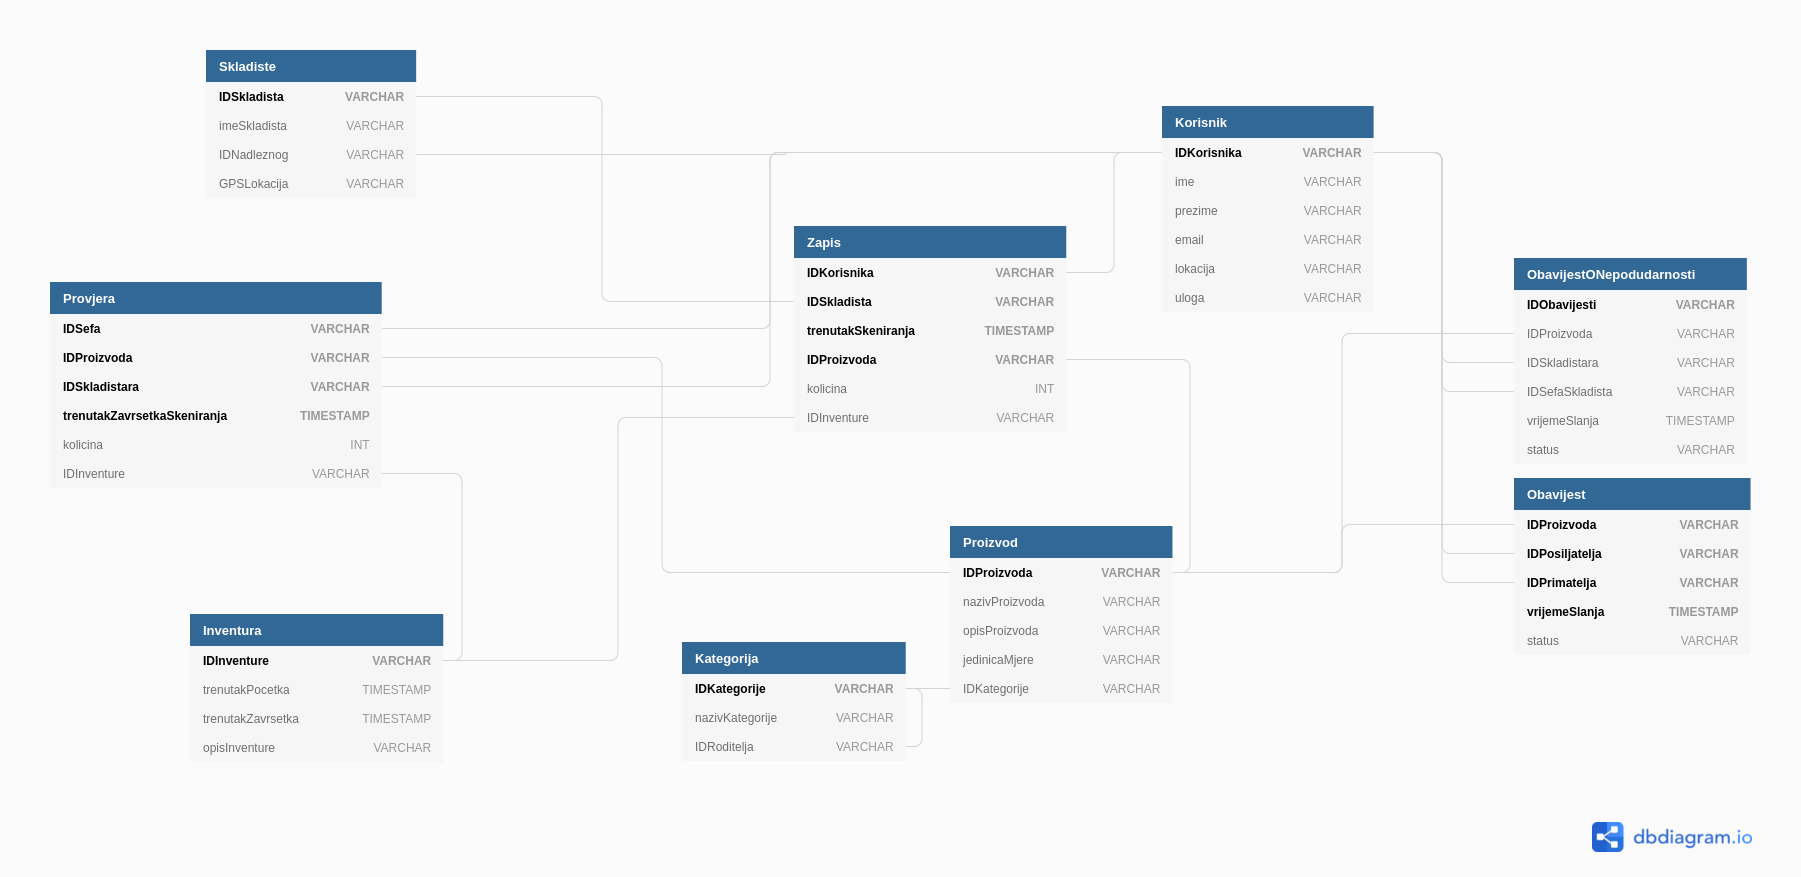
\includegraphics[scale=0.27]{"slike/ER_slika.png"}
					\caption{ER dijagram baze podataka}
					\label{Slika 4.1}
				\end{figure}
			
			\eject
			
			
		\section{Dijagram razreda}
			
			\begin{comment}
			\textbf{\textit{dio 1. revizije}}\\
			
			\textit{Prilikom prve predaje projekta, potrebno je priložiti potpuno razrađen dijagram razreda vezan uz \textbf{generičku funkcionalnost} sustava. Ostale funkcionalnosti trebaju biti idejno razrađene u dijagramu sa sljedećim komponentama: nazivi razreda, nazivi metoda i vrste pristupa metodama (npr. javni, zaštićeni), nazivi atributa razreda, veze i odnosi između razreda.}\\
			\end{comment}
			
			Na slikama 4.2 i 4.3 prikazani su razredi koji pripadaju backend dijelu aplikacije. Razredi sa slike 4.2 nasljeđuju razred Person i implementiraju dodatne potrebne metode. Razred Person sadrži još dodatno atribut role, koji je po tipu enumeracija Role. Slika 4.3 prikazuje odnose razreda koji se međusobno ne nasljeđuju.
			\begin{figure}[H]
				\centering
				\includegraphics[width=1.0\linewidth]{"slike/Class Diagram0"}
				\caption{Dijagram razreda - razredi koji nasljeđuju razred Person}
				\label{Slika 4.2}
			\end{figure}
			
			\begin{figure}[H]
				\centering
				\includegraphics[width=1.0\linewidth]{"slike/Class Diagram1"}
				\caption{Dijagram razreda - odnosi među klasama}
				\label{Slika 4.3}
			\end{figure}
			
			Svi razredi prikazani na slici 4.3 komuniciraju s bazom podataka kako bi dohvatili i spremili potrebne atribute. Razred Director ima najveće ovlasti. Nakon njega ide razred Manager, pa nakon njega Worker.
			
			\begin{comment}
			\textbf{\textit{dio 2. revizije}}\\			
			
			\textit{Prilikom druge predaje projekta dijagram razreda i opisi moraju odgovarati stvarnom stanju implementacije}
			\end{comment}
			
			
			\eject
		
		\section{Dijagram stanja}
			
			\begin{comment}
			
			\textbf{\textit{dio 2. revizije}}\\
			
			\textit{Potrebno je priložiti dijagram stanja i opisati ga. Dovoljan je jedan dijagram stanja koji prikazuje \textbf{značajan dio funkcionalnosti} sustava. Na primjer, stanja korisničkog sučelja i tijek korištenja neke ključne funkcionalnosti jesu značajan dio sustava, a registracija i prijava nisu. }
			
			\end{comment}
		
			\begin{figure}[H]
				\centering
				\includegraphics[width=1.0\linewidth]{"slike/Dijagram stanja"}
				\caption{Dijagram stanja - paljenje kamere i skeniranje artikala}
				\label{Slika 4.4}
			\end{figure}
		
			Slika 4.4 prikazuje dijagram stanja aplikacije prilikom pokretanja kamere. Prvi zadatak aplikacije je pokrenuti kameru na uređaju korisnika. Ukoliko pokretanje kamere nije moguće, dojavljuje se pogreška i izlazi se iz prozora. Ako je kamera uspješno pokrenuta, korisnik započinje skeniranje artikla. Najprije se dohvaćaju podaci o artiklu iz baze podataka i prikazuju se korisniku. Zatim, korisnik ažurira vrijednosti artikala te se, prilikom dovršetka rada, promjene spremaju u bazu podataka i kamera se gasi.
			
			\eject 
		
		
		\section{Dijagram aktivnosti}
			
			\begin{comment}
				\textbf{\textit{dio 2. revizije}}\\
				
				\textit{Potrebno je priložiti dijagram aktivnosti s pripadajućim opisom. Dijagram aktivnosti treba prikazivati značajan dio sustava.}
			\end{comment}
		
			\begin{figure}[H]
				\centering
				\includegraphics[width=1.0\linewidth]{"slike/Dijagram aktivnosti"}
				\caption{Dijagram aktivnosti - skeniranje artikla i komunikacija s bazom podataka}
				\label{Slika 4.5}
			\end{figure}
			
			Slika 4.5 prikazuje paljenje kamere i ažuriranje podataka o skeniranom artiklu u bazi podataka. Prvo se provjerava status kamere. Ukoliko se kamera nije uspjela pokrenuti, prekida se proces skeniranja artikla. Ako se kamera pokrenula, uspostavlja se veza s bazom podataka, kako bi korisnik mogao dohvatiti podatke o skeniranom artiklu. Ukoliko se veza s bazom podataka nije uspjela uspostaviti, prekida se proces skeniranja artikla. U suprotnom, baza podataka vraća podatke o traženom artiklu te se ti podaci prikazuju korisniku u obliku pop-up screena. Korisnik tu unosi nove vrijednosti, koje se u bazu podataka spremaju na dva načina: nakon isteka vremena od 5 sekundi ili kada korisnik pritisne gumb "Spremi". Korisnik također može prekinuti skeniranje artikla u bilo kojem trenutku, pritiskom bilo gdje na ekran uređaja, prilikom čega se odbacuju izmjene. Na kraju, ukoliko se podaci nisu uspjeli spremiti u bazu, gasi se skeniranje artikala. Ukoliko su podaci uspješno spremljeni, aplikacija završava normalno s radom i korisnik može započeti novo skeniranje artikla.
			
			\eject
			
		\section{Dijagram komponenti}
		
			\begin{comment}
				\textbf{\textit{dio 2. revizije}}\\
				
				\textit{Potrebno je priložiti dijagram komponenti s pripadajućim opisom. Dijagram komponenti treba prikazivati strukturu cijele aplikacije.}
			\end{comment}
		 	
		 	\begin{figure}[H]
		 		\centering
		 		\includegraphics[width=0.8\linewidth]{"slike/Dijagram komponenti"}
		 		\caption{Dijagram komponenti - struktura aplikacije}
		 		\label{Slika 4.6}
		 	\end{figure}
	 	
	 		Slika 4.6 prikazuje rad i komunikaciju između pojedinih komponenti aplikacije. Aplikacija je namijenjena za pokretanje na mobilnim uređajima, a pisana je u Flutteru. Podaci potrebni za rad aplikacije se dohvaćaju iz Firestore baze podataka.
			 